
\documentclass[11pt,a4paper]{report}%especifica o tipo de documento que tenciona escrever: carta, artigo, relatório... neste caso é um relatório
% [11pt,a4paper] Define o tamanho principal das letras do documento. caso não especifique uma delas, é assumido 10pt
% a4paper -- Define o tamanho do papel.

\usepackage[portuges]{babel}%Babel -- irá activar automaticamente as regras apropriadas de hifenização para a língua todo o
                                   %-- o texto gerado é automaticamente traduzido para Português.
                                   %  Por exemplo, “chapter” irá passar a “capítulo”, “table of contents” a “conteúdo”.
                                   % portuges -- específica para o Português.
\usepackage[utf8]{inputenc} % define o encoding usado texto fonte (input)--usual "utf8" ou "latin1

\usepackage{graphicx} %permite incluir graficos, tabelas, figuras
\usepackage{url} % para utilizar o comando \url{}
\usepackage{enumerate} %permite escolher, nas listas enumeradas, se os iems sao marcados com letras ou numeros-romanos em vez de numeracao normal

%\usepackage{apalike} % gerar biliografia no estilo 'named' (apalike)

\usepackage{color} % Para escrever em cores

\usepackage{multirow} %tabelas com multilinhas
\usepackage{array} %formatação especial de tabelas em array

\usepackage[pdftex]{hyperref} % transformar as referências internas do seu documento em hiper-ligações.

%Exemplos de fontes -- nao e vulgar mudar o tipo de fonte
%\usepackage{tgbonum} % Fonte de letra: TEX Gyre Bonum
%\usepackage{lmodern} % Fonte de letra: Latin Modern Sans Serif
%\usepackage{helvet}  % Fonte de letra: Helvetica
%\usepackage{charter} % Fonte de letra:Charter

\definecolor{saddlebrown}{rgb}{0.55, 0.27, 0.07} % para definir uma nova cor, neste caso 'saddlebrown'

\usepackage{listings}  % para utilizar blocos de texto verbatim no estilo 'listings'
%paramerização mais vulgar dos blocos LISTING - GENERAL
\lstset{
	basicstyle=\small, %o tamanho das fontes que são usadas para o código
	numbers=left, % onde colocar a numeração da linha
	numberstyle=\tiny, %o tamanho das fontes que são usadas para a numeração da linha
	numbersep=5pt, %distancia entre a numeração da linha e o codigo
	breaklines=true, %define quebra automática de linha
    frame=tB,  % caixa a volta do codigo
	mathescape=true, %habilita o modo matemático
	escapeinside={(*@}{@*)} % se escrever isto  aceita tudo o que esta dentro das marcas e nao altera
}
%
%\lstset{ %
%	language=Java,							% choose the language of the code
%	basicstyle=\ttfamily\footnotesize,		% the size of the fonts that are used for the code
%	keywordstyle=\bfseries,					% set the keyword style
%	%numbers=left,							% where to put the line-numbers
%	numberstyle=\scriptsize,				% the size of the fonts that are used for the line-numbers
%	stepnumber=2,							% the step between two line-numbers. If it's 1 each line
%											% will be numbered
%	numbersep=5pt,							% how far the line-numbers are from the code
%	backgroundcolor=\color{white},			% choose the background color. You must add \usepackage{color}
%	showspaces=false,						% show spaces adding particular underscores
%	showstringspaces=false,					% underline spaces within strings
%	showtabs=false,							% show tabs within strings adding particular underscores
%	frame=none,								% adds a frame around the code
%	%abovecaptionskip=-.8em,
%	%belowcaptionskip=.7em,
%	tabsize=2,								% sets default tabsize to 2 spaces
%	captionpos=b,							% sets the caption-position to bottom
%	breaklines=true,						% sets automatic line breaking
%	breakatwhitespace=false,				% sets if automatic breaks should only happen at whitespace
%	title=\lstname,							% show the filename of files included with \lstinputlisting;
%											% also try caption instead of title
%	escapeinside={\%*}{*)},					% if you want to add a comment within your code
%	morekeywords={*,...}					% if you want to add more keywords to the set
%}

\usepackage{xspace} % deteta se a seguir a palavra tem uma palavra ou um sinal de pontuaçao se tiver uma palavra da espaço, se for um sinal de pontuaçao nao da espaço

\parindent=0pt %espaço a deixar para fazer a  indentação da primeira linha após um parágrafo
\parskip=2pt % espaço entre o parágrafo e o texto anterior

\setlength{\oddsidemargin}{-1cm} %espaço entre o texto e a margem
\setlength{\textwidth}{18cm} %Comprimento do texto na pagina
\setlength{\headsep}{-1cm} %espaço entre o texto e o cabeçalho
\setlength{\textheight}{23cm} %altura do texto na pagina

% comando '\def' usado para definir abreviatura (macros)
% o primeiro argumento é o nome do novo comando e o segundo entre chavetas é o texto original, ou sequência de controle, para que expande
\def\darius{\textsf{Darius}\xspace}
\def\antlr{\texttt{AnTLR}\xspace}
\def\pe{\emph{Publicação Eletrónica}\xspace}
\def\titulo#1{\section{#1}}    %no corpo do documento usa-se na forma '\titulo{MEU TITULO}'
\def\super#1{{\em Supervisor: #1}\\ }
\def\area#1{{\em \'{A}rea: #1}\\[0.2cm]}
\def\resumo{\underline{Resumo}:\\ }

%\input{LPgeneralDefintions} %permite ler de um ficheiro de texto externo mais definições

\title{Processamento de Linguagens e Compiladores (3º ano de Curso)\\
       \textbf{Trabalho Prático nº 1
}\\ Relatório de Desenvolvimento\\-----------
\\Grupo nr. 15

       } %Titulo do documento
%\title{Um Exemplo de Artigo em \LaTeX}
\author{Ruben Silva\\ (a94633) \and Carlos Costa\\ (a94543)
       } %autores do documento
\date{\today} %data

\begin{document} % corpo do documento
\maketitle % apresentar titulo, autor e data

\begin{abstract}  % resumo do documento
Neste relatório encontra-se a resolução do Trabalho Prático 1 mais
precisamente os exercícios 1 e 2 do respetivo enunciado de 2022 para 
a unidade curricular Processamento de Linguagens e Compiladores.\\
O objetivo deste trabalho é a utilização de expressões regulares (ER) para transformação de texto bem como processos de filtragem entre outros.\\\
\end{abstract}

\tableofcontents % Insere a tabela de indice
%\listoffigures % Insere a tabela de indice figuras
%\listoftables % Insere a tabela de indice tabelas

\chapter{Processador de Pessoas listadas nos Róis de Confessados} \label{chap:ex1} %referência cruzada

\section{Análise do Problema 1} \label{sec:analiseProb1}

Neste problema recebemos 1 ficheiro que continha algumas informações sobre uns processos de pessoas listadas nos róis de confessados. Estas  estavam claramente divididas pela expressão "::".
O objetivo deste problema era obter:

\begin{itemize}
  \item A frequência de processos por ano (primeiro elemento da data);
  \item A frequência de nomes próprios (o primeiro em cada nome) e apelidos (o ultimo em cada nome) por séculos;
  \item A frequência dos vários tipos de relação: irmão, sobrinho, etc.
  \item Obter um ficheiro JSON com os primeiros 20 registos desse ficheiro.
\end{itemize}

Na seguinte figura podemos ver um excerto desse ficheiro:\\
\begin{figure}[htbp]
\centerline{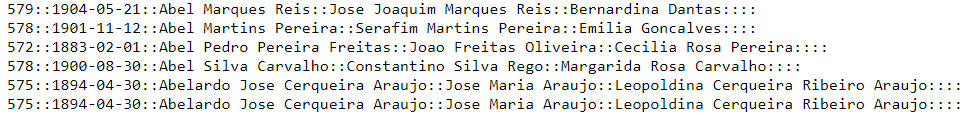
\includegraphics{exemploProcessos.png}}
\caption{Excerto do ficheiro processos.txt}
\label{fig}
\end{figure}

Cada coluna tinha respetivamente as seguintes informações:

\begin{itemize}
  \item Coluna 1/2/3: Pasta::Data::Nome;
  \item Coluna 4/5: Pai/Mãe;
  \item Coluna 6: Observação.
\end{itemize}


\section{Resolução do Problema 1} \label{sec:resProb1}

Para a resolução deste problema recorremos às seguintes soluções sequenciadas:

\begin{enumerate}[i)]
     \item Criar um dicionário e alocar cada processo com as respetivas informações;
     \item Processar cada frequência individualmente; 
     \item Criar o JSON;
  \end{enumerate}
  
  
  
\subsection{Alocar no Dicionário} \label{subsec:parser1}
Esta parte do problema foi resolvido com a função chamada filtrar\textunderscore info\\
Esta função inicialmente percorre o "file descriptor" do "processos.txt" que foi entregue por parâmetros e dá split ao código por linhas. Após isso é gerado uma lista que será percorrida novamente e levará outro split por cada vez que a expressão "::" aparecer e, claramente, se a linha não estiver vazia.\\
Após isso, é inicializada um dicionário que contém todas as informações necessárias para a realização deste problema.


\begin{figure}[htbp]
\centerline{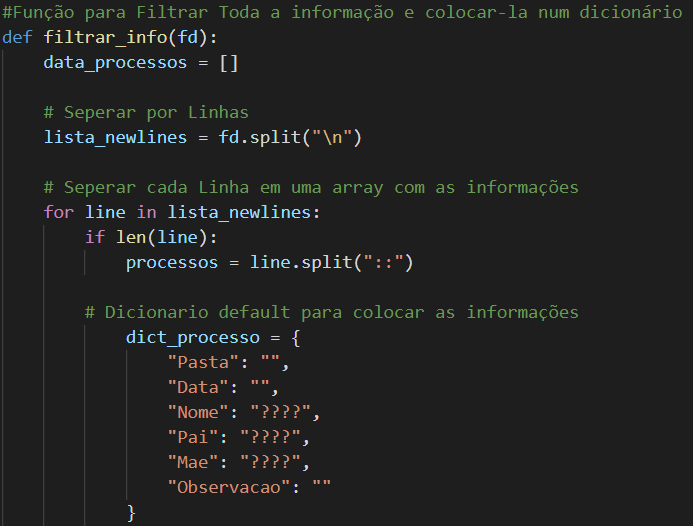
\includegraphics{filtra_info1_EX1.png}}
\caption{Excerto da função filtrar\textunderscore info(fd) PARTE 1}
\label{fig}
\end{figure}  

Como visto na figura anterior, cada informação do nosso problema, agora numa lista criada pelo split, e chamada "paramatro", será processada pelas Expressões Regulares (ER):


\begin{itemize}
  \item ER Data: \texttt{"[0-9]{4}-[0-9]{1,2}-[0-9]{1,2}"};
  \item ER Numero da Pasta: \texttt{"[0-9]{1,4}"};
  \item ER que verifica se existe palavras com letras maiúsculas: \texttt{"([A-Z]{1}[a-z]* ?)"};
  \item ER que verifica se é uma observação: \texttt{"[\textasciicircum A-Z]{1}\textbackslash ."} .
\end{itemize}

Inicialmente, passa pelas ER da data e do nr da pasta que são as mais fáceis de identificar. Após isso, queremos encontrar a existência de letras maiúsculas nessa informação, se existir, então queremos encontrar uma letra maiúscula seguida de um ponto final, se isto acontecer, claramente é uma observação.\\
A alocação do Nome, Pai, Mãe é feita ordenadamente consoante o seu preenchimento no dicionário, pois eles aparecem de forma ordenada no ficheiro processos. Para conseguirmos isso, simplesmente vamos identificando se já foi ou não alocado. Como ultima alocação, se informação não se identificar com nenhumas das ER e ser igual a (""), então essa informação não existe e convém marcar-la de algum modo.\\

Após esta verificação em cada umas ER anteriores, é alocado devidamente no dicionário e posteriormente metido numa lista para return

\begin{figure}[htbp]
\centerline{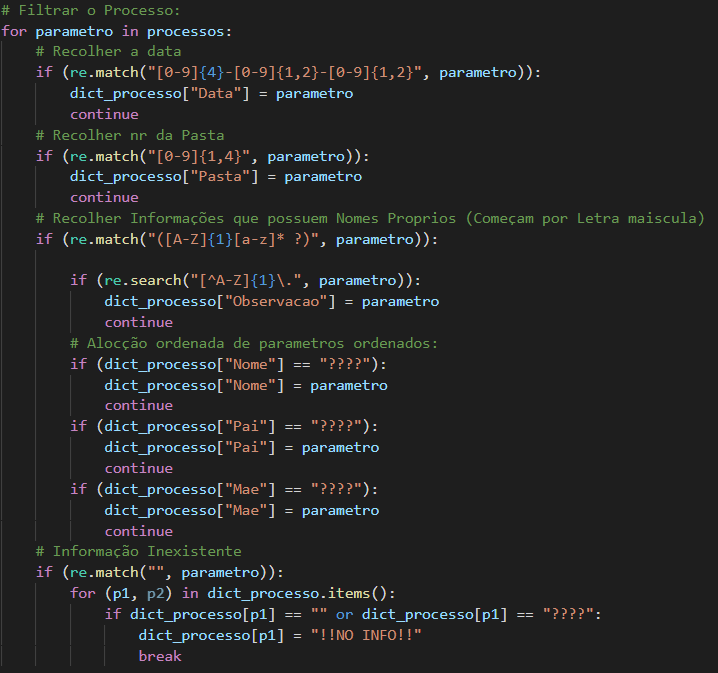
\includegraphics{filtra_info2_EX1.png}}
\caption{Excerto da função filtrar\textunderscore info(fd) PARTE 2}
\label{fig}
\end{figure} 

\subsection{Cálculo das Frequências} \label{subsec:freqCalc}
Esta parte do problema foi resolvido com 3 funções distintas: calcular\textunderscore freq\textunderscore processos, calcular\textunderscore freq\textunderscore nomes\textunderscore sec, calcular\textunderscore freq\textunderscore relacao.\\

\title{\textbf{calcular\textunderscore freq\textunderscore processos(data)}}

Nesta função era necessário calcular a frequência de processos por ano.\\
A nossa solução para este problema foi a criação de um dicionário auxiliar e uma pesquisa na nossa estrutura de dados que irá alocar nesse dicionário todos os processos de cada ano especifico.\\
Para a recolha do ano, usamos uma expressão regular que simplesmente pega no único valor com 4 dígitos (ano).\\
Após isto, a nossa nova data foi tabelada de forma ordenada.\\
A fórmula matemática para esta frequência foi:  \\

$$
\texttt { Frequência }=\frac{\texttt { Processos de um Certo Ano }}{\texttt { Todos os Processos }}
$$





\begin{figure}[htbp]
\centerline{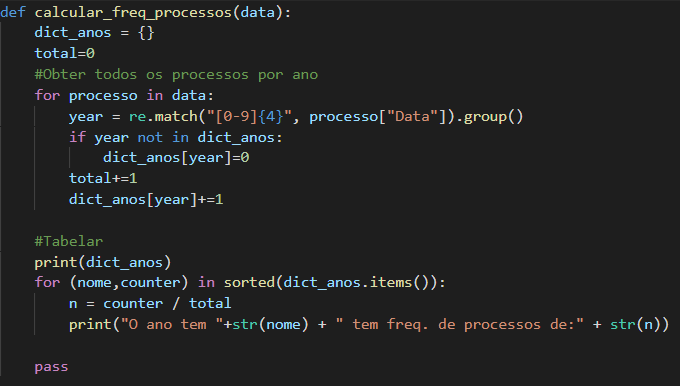
\includegraphics{calc_freq_processos.png}}
\caption{Função calc\textunderscore freq\textunderscore processos(data)}
\label{fig}
\end{figure}  

\newpage
\title{\textbf{calcular\textunderscore freq\textunderscore nomes\textunderscore sec(data)}}

Nesta função era necessário calcular a frequência de nomes por século.\\
Esta funciona foi de longe a mais complexa porque tivemos de filtrar os nomes que constavam nas observações\\
A nossa solução para este problema foi a criação de dois dicionários auxiliares (nomes e apelidos) e uma pesquisa na nossa estrutura de dados que irá alocar nesses dicionários todos os nomes e apelidos de cada século.\\
Para a recolha do século, usamos uma expressão regular que simplesmente pega no único valor com 4 dígitos (ano) e aplicamos-lhe a seguinte formula matemática:
$$
\texttt { Século }=\frac{\texttt { (Ano - 1) }}{\texttt { 100 }} + 1
$$
\begin{figure}[htbp]
\centerline{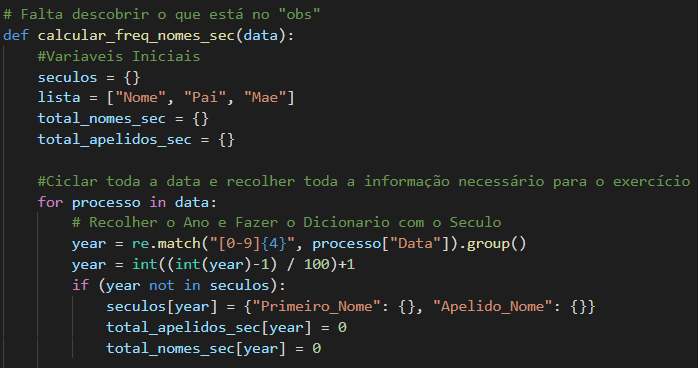
\includegraphics{calc_freq_nomes_sec1.png}}
\caption{Excerto da Função calc\textunderscore freq\textunderscore nomes\textunderscore sec(data) PARTE 1}
\label{fig}
\end{figure} 

Numa segunda parte desta função, tivemos de recolher os nomes e os apelidos de cada processo.
Para isto, percorremos os processos e filtrávamos o pretendido com ER.
Inicialmente, ao percorrer os nossos dados, usamos uma ER para recolhemos logo o primeiro nome: (ER Numero da Pasta: \texttt{"[0-9]{1,4}"}).\\
Para recolhermos o apelido, tivemos bastante mais trabalho, pois muitos nomes, não eram uniformes, por exemplo:

 \begin{figure}[htbp]
\centerline{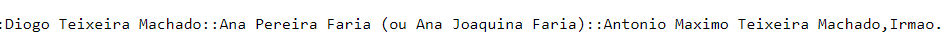
\includegraphics{exemploProcessos_apelido.png}}
\caption{Exemplo de um Processo com o nome irregular}
\label{fig}
\end{figure}

Para este caso especifico, simplesmente criamos duas ER que encontrava o parêntese "(" , ")" e a partir dai extraiamos os dois possíveis apelidos.\\
Tivemos outro caso muito irregular também, em que continha uma virgula, por exemplo: "Maria Vale, Solteira". Para este caso também criamos uma ER que recolhia a palavra antes da vírgula.\\


\begin{figure}[htbp]
\centerline{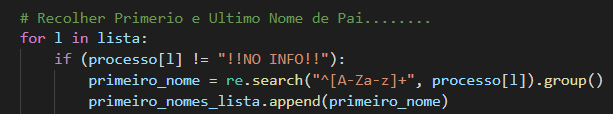
\includegraphics{calc_freq_nomes_sec21.png}}
\caption{Excerto da Função calc\textunderscore freq\textunderscore nomes\textunderscore sec(data) PARTE 2.1}
\label{fig}
\end{figure}
\begin{figure}[htbp]
\centerline{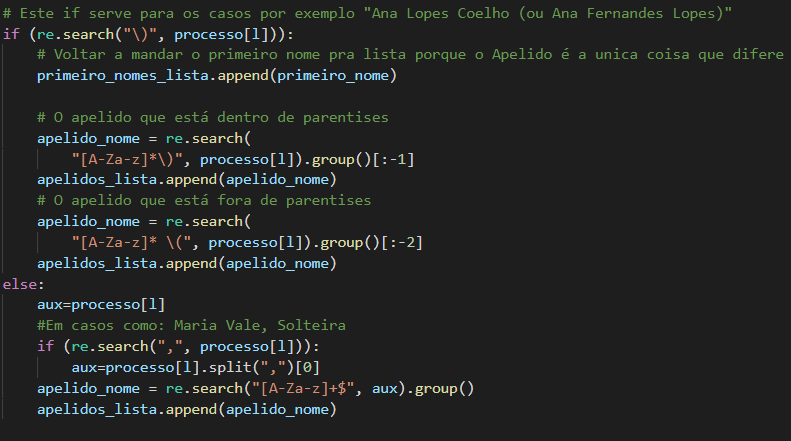
\includegraphics{calc_freq_nomes_sec22.png}}
\caption{Excerto da Função calc\textunderscore freq\textunderscore nomes\textunderscore sec(data) PARTE 2.2}
\label{fig}
\end{figure}

Neste excerto da função, filtramos o que estava na observação.
Para isso criamos inicialmente uma ER que encontra um nome seguido de vírgula (o padrão que encontramos para este filtro) (ER = \texttt{"(([A-Z]{1}[a-z]{1,} ?)+\,)"}
Após encontrarmos esse nome, aplicávamos as ER normais para obter o nome e o apelido.\\
\begin{figure}[htbp]
\centerline{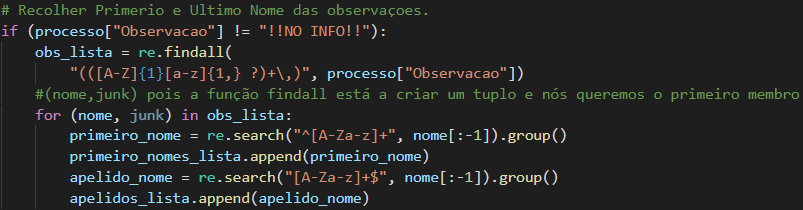
\includegraphics{calc_freq_nomes_sec3.png}}
\caption{Excerto da Função calc\textunderscore freq\textunderscore nomes\textunderscore sec(data) PARTE 3}
\label{fig}
\end{figure}
\\No final destas filtragens, simplesmente metemos dentro dos dicionário inicialmente criados e aplicamos a seguinte formula matemática a cada século:
$$
\texttt { Frequência }=\frac{\texttt { Número de Certo Nome desse Século }}{\texttt { Todos os Nomes desse Século }}
$$

Por fim, esses valores foram tabelados no output.

\begin{figure}[htbp]
\centerline{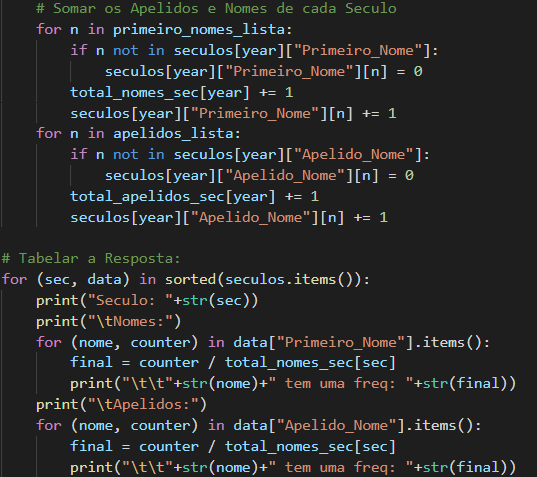
\includegraphics{calc_freq_nomes_sec4.png}}
\caption{Excerto da Função calc\textunderscore freq\textunderscore nomes\textunderscore sec(data) PARTE 4}
\label{fig}
\end{figure}


\title{\textbf{calcular\textunderscore freq\textunderscore relacao(data)}}\\
Nesta função era necessário calcular a frequência de relações.\\
A nossa solução para este problema foi a criação de um dicionário que guardará o nr de cada relação existente.
No inicio da função, simplesmente percorremos os nossos dados e vamos somando ao dicionário sempre que existe mãe ou pai.\\

\begin{figure}[htbp]
\centerline{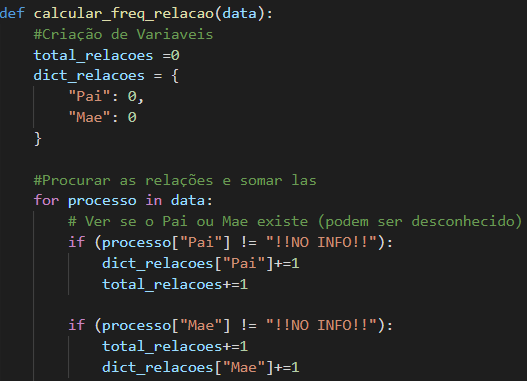
\includegraphics{calc_freq_relacao1.png}}
\caption{Excerto da Função calc\textunderscore freq\textunderscore relacao(data) PARTE 1}
\label{fig}
\end{figure}

Nesta parte da função, temos de encontrar as relações que estão presentes da observação e com para esse objetivo conseguimos encontrar um padrão após a virgula e a partir dai chegar à ER = "\texttt{"[\textasciicircum A-Z]\,(([A-Z]{1}[a-z ]+)+)\."}.
Mas contudo, tivemos 2 casos que não se encaixavam neste padrão, e como tal, tivemos de os excluir.
\begin{figure}[htbp]
\centerline{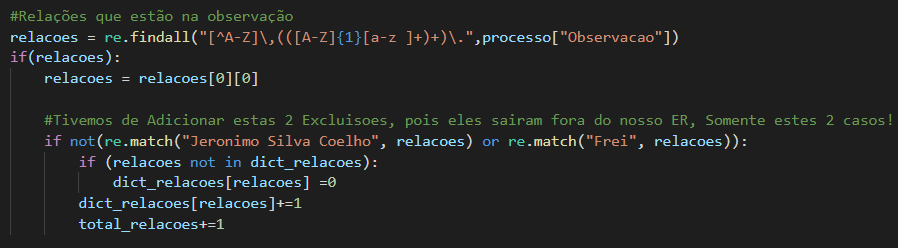
\includegraphics{calc_freq_relacao2.png}}
\caption{Excerto da Função calc\textunderscore freq\textunderscore relacao(data) PARTE 2}
\label{fig}
\end{figure}

No fim de tudo, tabelamos o resultado
\begin{figure}[htbp]
\centerline{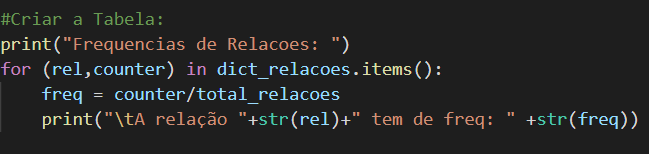
\includegraphics{calc_freq_relacao3.png}}
\caption{Excerto da Função calc\textunderscore freq\textunderscore relacao(data) PARTE 2}
\label{fig}
\end{figure}


\subsection{Criar o JSON} \label{subsec:jsondump}
Esta parte do problema, foi a mais simples de toda, pois já tínhamos os processos todos tratados devidamente.\\
Simplesmente criamos uma função que "junta" o nosso dicionário a uma lista básica que  é normalmente usada em ficheiros JSON.

\begin{figure}[htbp]
\centerline{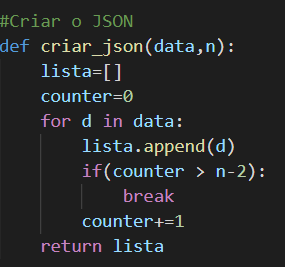
\includegraphics{criar_JSON.png}}
\caption{Função que cria o JSON}
\label{fig}
\end{figure}

\newpage
\section{Resultados do Problema 1} \label{sec:resProb1}
\subsection{Resultado da Frequência de Processos por Ano} \label{subsec:resProcAno}

Aqui temos um excerto, devido ao output ser extenso, do resultado da Frequência de Processos por Ano.

\begin{figure}[htbp]
\centerline{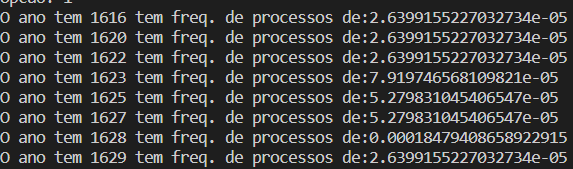
\includegraphics{resProcAno.png}}
\caption{Excerto do Resulto da freq. de Processos por Ano}
\label{fig}
\end{figure}


\subsection{Resultado da Frequência de Nomes e Apelidos por Século} \label{subsec:resNomeSec}

Aqui temos um excerto, devido ao output ser extenso, do resultado Frequência de Nomes e Apelidos por Século.

\begin{figure}[htbp]
\centerline{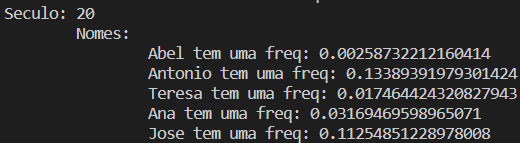
\includegraphics{resNomeSec.png}}
\caption{Excerto do Resulto da freq. Nomes e Apelidos por Século}
\label{fig}
\end{figure}


\newpage
\subsection{Resultado da Frequência de Relações} \label{subsec:resRel}


\begin{figure}[htbp]
\centerline{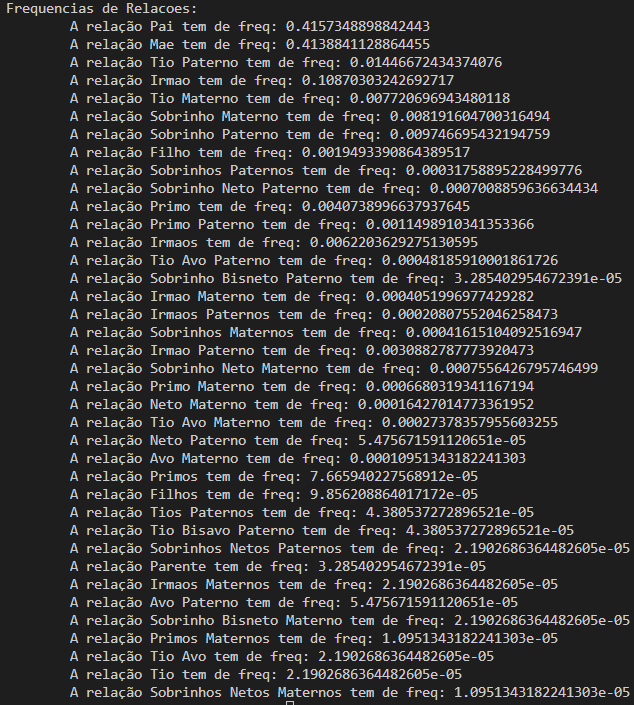
\includegraphics{resRel.png}}
\caption{Resulto de freq. de Relações}
\label{fig}
\end{figure}

\newpage

\section{Main} \label{sec:main1}

Por fim, achamos necessário abrir o ficheiro "processos.txt" e criar um menu para escolhermos qual das frequências imprimir na consola. Após o processamento de tudo, é executada a função que irá gerar o JSON com os primeiro 20 processos.

\begin{figure}[htbp]
\centerline{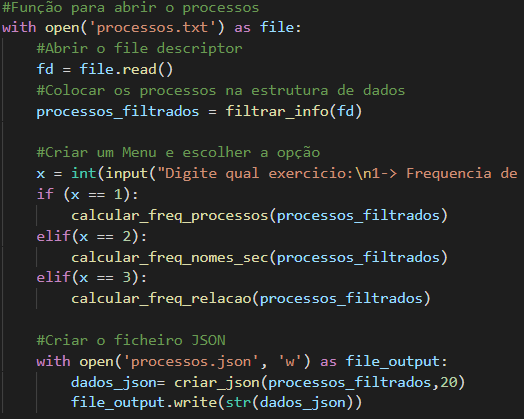
\includegraphics{mainEx1.png}}
\caption{Código da main}
\label{fig}
\end{figure}

Na imagem abaixo encontra-se o menu do nosso código.
\begin{figure}[htbp]
\centerline{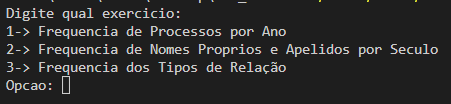
\includegraphics{menuEx1.png}}
\caption{Menu do Problema}
\label{fig}
\end{figure}


\newpage
\chapter{ Processador de Registos de Exames Médicos Desportivos} \label{chap:ex2} %capitulo e referencia cruzada


\section{Análise do Problema 2} \label{sec:analiseProb2}
Neste problema recebemos um "dataset" gerado no âmbito do registo de exames médicos desportivos.
O objetivo deste problema era obter:

\begin{itemize}
  \item Datas extremas dos registos no dataset;
  \item Distribuição por modalidade em cada ano e no total;
  \item Distribuição por idade e género (para a idade, considera apenas 2 escalões: < 35 anos e >= 35);
  \item Distribuição por morada;
  \item Percentagem de aptos e não aptos por ano.
\end{itemize}

E num segundo parâmetro, era requerido a listagem de todos os dados usados para cada uma dos indicadores gerados.

Na seguinte figura podemos ver um excerto desse ficheiro:\\
\begin{figure}[htbp]
\centerline{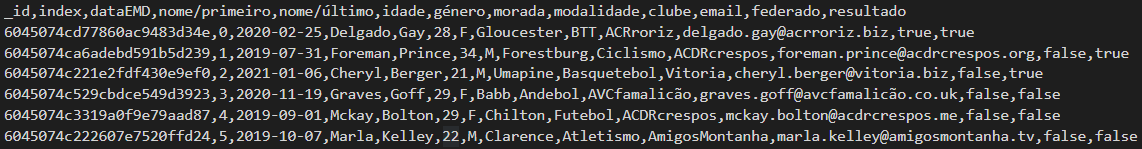
\includegraphics[scale=0.8]{exemploCSVDesporto.png}}
\caption{Excerto do ficheiro emd.csv}
\label{fig}
\end{figure}

\newpage
\section{Resolução do Problema 2} \label{sec:resProb2}

Para a resolução deste problema recorremos às seguintes soluções sequenciadas:

\begin{enumerate}[i)]
     \item Criar um dicionário e alocar cada processo com as respetivas informações;
     \item Calcular cada indicador individualmente; 
     \item Desenhar a tabela de cada indicador individualmente em html
     \item Gerar a lista de dados usados para cada indicador individualmente em html
	 \item Gerar todos os ficheiros HTML com todos os dados devidamente processados
  \end{enumerate}
  
  
  
\subsection{Alocar no Dicionário} \label{subsec:parser2}
Esta parte do problema foi resolvido com a função chamada filtrar\textunderscore csv\\
Esta função inicialmente percorre o "file descriptor" do "processos.txt" que foi entregue por parâmetros e dá split ao código por linhas. Após isso é gerado uma lista que será percorrida novamente e levará outro split por cada vez que a expressão "," aparecer.\\
Após isso, é inicializada um dicionário que contém todas as informações necessárias para a realização deste problema.

\begin{figure}[htbp]
\centerline{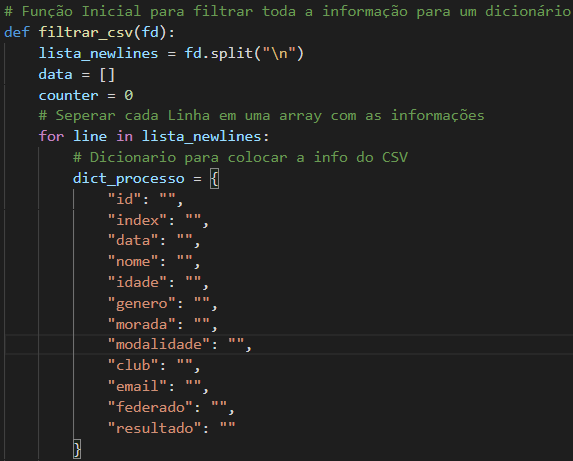
\includegraphics{filtra_info1_EX2.png}}
\caption{Excerto da função filtrar\textunderscore csv(fd) PARTE 1}
\label{fig}
\end{figure}  

Como visto na figura anterior, cada informação do nosso problema, agora numa lista criada pelo split, e chamada "row", será processada pelas Expressões Regulares (ER):


\begin{itemize}
  \item ER Id: \texttt{"[0-9a-z]{24}"};
  \item ER Index: \texttt{"[0-9]{1,2}"};
  \item ER Data: \texttt{"[0-9]{4}-[0-9]{1,2}-[0-9]{1,2}"};
  \item ER Nome|Morada|Modalidade|Club: \texttt{"[A-Za-z]+"};
  \item ER Idade: \texttt{"[0-9]{2}"};
  \item ER Género: \texttt{"[MF]{1}"};
  \item ER Email: \texttt{"[a-zA-Z.]+@[a-zA-Z.]+"};
  \item ER Numero da Pasta: \texttt{"[0-9]{1,4}"};
  \item ER Federado|Resultado: \texttt{"[true|false]"};
\end{itemize}

Cada Coluna da linha (membro da lista) é processado diretamente pela respetiva coluna (pois o dataset é perfeitamente ordenado).
Fazemos a verificação com as ERs para evitar dados anormais.

\begin{figure}[htbp]
\centerline{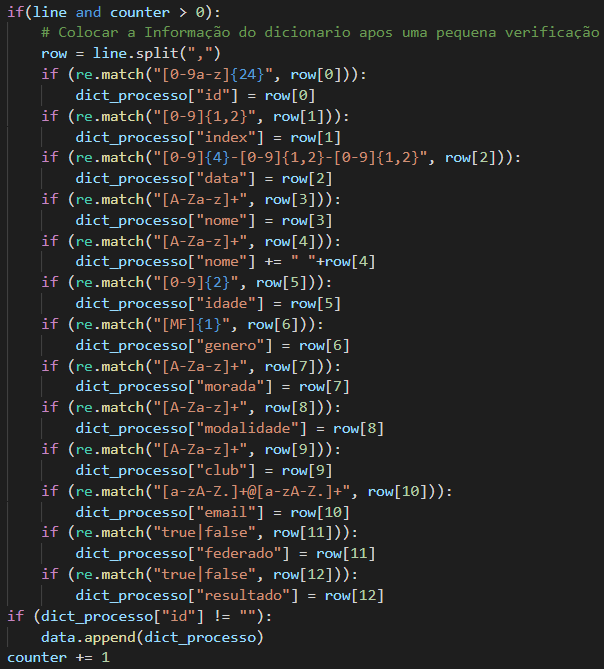
\includegraphics{filtra_info2_EX2.png}}
\caption{Excerto da função filtrar\textunderscore csv(fd) PARTE 2}
\label{fig}
\end{figure} 



\subsection{Cálculo dos Indicadores} \label{subsec:indicadoresCalc}
Esta parte do problema foi resolvido com 5 funções distintas: datas\textunderscore extremas, distribuicao\textunderscore modalidade\textunderscore ano, distribuicao\textunderscore modalidade\textunderscore ano,distribuicao\textunderscore morada,aptos.\\

\title{\textbf{datas\textunderscore extremas(data)}}

Nesta função era necessário simplesmente pegar no ano de cada processo e colocar-los numa lista para ordenar-la por ordem crescente (sort).\\
Após isso, pegamos no primeiro membro dessa lista (menor data) e o último membro dessa lista (maior data).\\
No final damos return a um tuplo com as datas extremas.



\begin{figure}[htbp]
\centerline{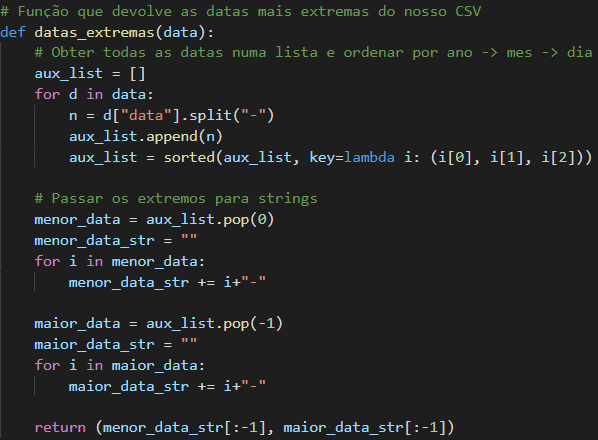
\includegraphics{datas_extremas.png}}
\caption{Função datas\textunderscore extremas(data)}
\label{fig}
\end{figure}  

\newpage
\title{\textbf{distribuicao\textunderscore modalidade \textunderscore ano(data)}}

Nesta função era necessário pegar no ano de cada processo e criar um dicionário com as chaves são os anos e os valores são as modalidades que estas últimas, possuem contadores.\\

\begin{figure}[htbp]
\centerline{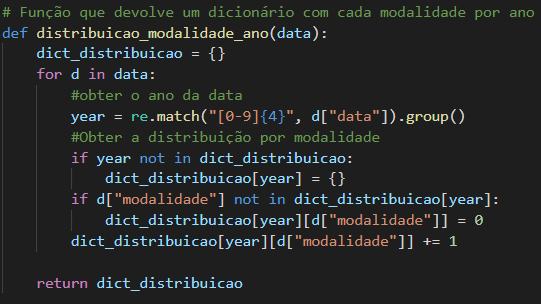
\includegraphics{distribuicao_modalidade_ano.png}}
\caption{Função distribuicao\textunderscore modalidade \textunderscore ano(data)}
\label{fig}
\end{figure}  

\title{\textbf{distribuicao\textunderscore modalidade \textunderscore ano(data)}}

Nesta função era necessário pegar nas idades de cada processo e criar um dicionário com as chaves são é a idade e os valores são o sexo e estas últimas, possuem contadores.\\
Numa segunda parte, ao mesmo tempo que é filtrado a idade, também adicionamos os escalões.
\begin{figure}[htbp]
\centerline{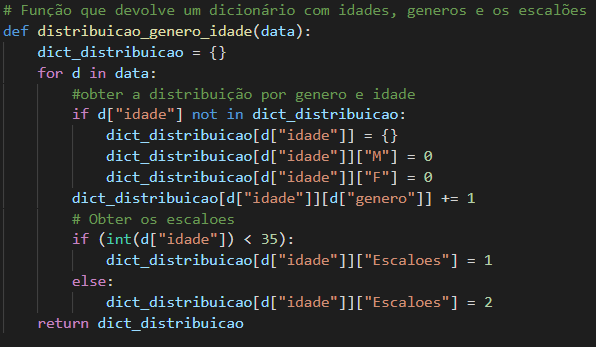
\includegraphics{distribuicao_genero_idade.png}}
\caption{Função distribuicao\textunderscore genero \textunderscore idade(data)}
\label{fig}
\end{figure}  

\newpage
\title{\textbf{distribuicao\textunderscore morada(data)}}

Nesta função era necessário pegar nas moradas de cada processo e criar um dicionário com as chaves são é a morada e os valores os contadores.\\
\begin{figure}[htbp]
\centerline{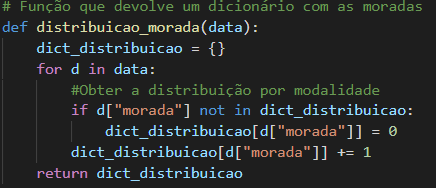
\includegraphics{distribuicao_morada.png}}
\caption{Função distribuicao\textunderscore morada(data)}
\label{fig}
\end{figure} 

\title{\textbf{aptos(data)}}

Nesta função, numa primeira parte era necessário pegar no ano de cada processo e criar um dicionário com as chaves são é o resultado e os valores "true" ou "false" e estas últimas, possuem contadores.\\
Numa segunda parte, é criado a percentagem com este dicionário.
\begin{figure}[htbp]
\centerline{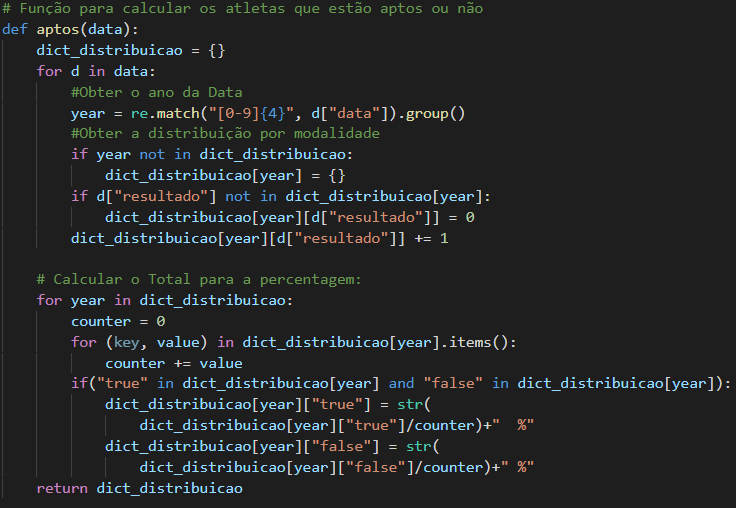
\includegraphics{aptos.png}}
\caption{Função aptos(data)}
\label{fig}
\end{figure}  



\newpage
\subsection{Tabela dos indicadores} \label{subsec:indicadoresTable}
Esta parte do problema foi resolvido com 4 funções distintas: draw\textunderscore table \textunderscore hmtl, draw\textunderscore table\textunderscore html\textunderscore morada, datas\textunderscore extremas\textunderscore html, indicadores\\

\title{\textbf{draw\textunderscore table\textunderscore html(data)}}

Esta função é a responsável por desenhar as tabelas dos indicadores mais gerais (género e idade, modalidade, aptos).
Esta função recebe alguns parâmetros para poder escrever o HTML (estes estão descritos no comentário da função).\\
Resumidamente, é criado uma tabela simples com os dados do dicionário e as tags do html são alocadas em strings criando assim um string gigante que será o suficiente para gerar o nosso html.\\
Essa string é depois substituída na string principal do html onde fica a tag "<body>".


\begin{figure}[htbp]
\centerline{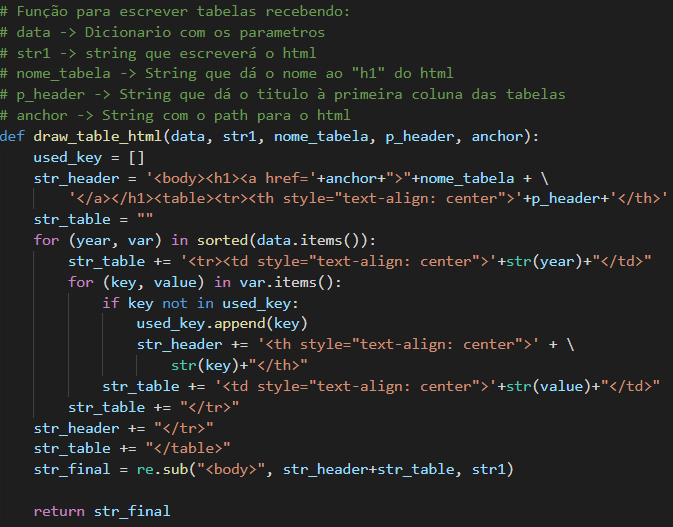
\includegraphics{draw_table_html.png}}
\caption{Função draw\textunderscore table \textunderscore hmtl(data, str1, nome\textunderscore tabela, p\textunderscore header, anchor)}
\label{fig}
\end{figure}  

\newpage
\title{\textbf{draw\textunderscore table\textunderscore html\textunderscore morada(data)}}

Esta função é basicamente igual à anterior, mas como o dicionário gerado pela função relativa à distribuição da morada tinha uma estrutura ligeiramente diferente, esta função teve de ser adaptada.


\begin{figure}[htbp]
\centerline{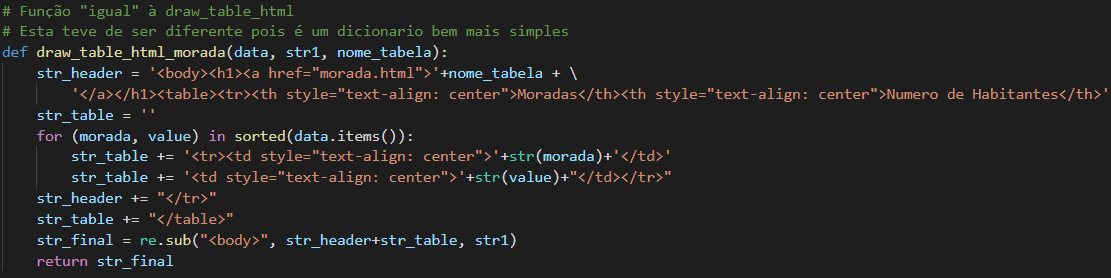
\includegraphics[scale=0.8]{draw_table_html_morada.png}}
\caption{Função draw\textunderscore table \textunderscore html(data, str1, nome\textunderscore tabela)}
\label{fig}
\end{figure}  


\title{\textbf{datas\textunderscore extremas\textunderscore html\textunderscore morada(data)}}

Esta função simplesmente cria uma pequena tabela com as 2 datas do tuplo.


\begin{figure}[htbp]
\centerline{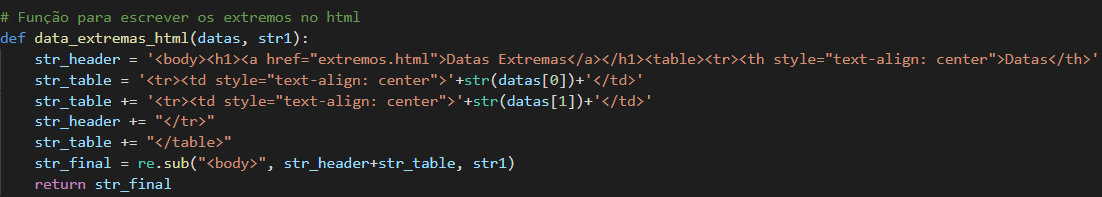
\includegraphics[scale=0.8]{datas_extremas_html.png}}
\caption{Função datas\textunderscore extremas \textunderscore html(data, str1)}
\label{fig}
\end{figure}


\newpage
\title{\textbf{indicadores(data,str1)}}

Esta função recebe a string principal para gerada o html e data.\\
Ela irá executar cada uma das de calcular as distribuições, percentagens... e irá adicionar à string principal cada uma das tabelas que irão ser obtidas também pela execução das respetivas funções de criação delas.\\
No fim, retornará a string principal para gerar o ficheiro html.


\begin{figure}[htbp]
\centerline{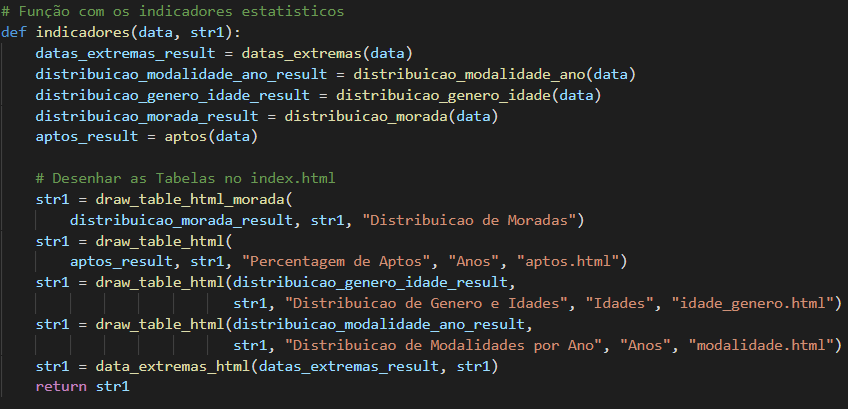
\includegraphics[scale=0.8]{indicadores.png}}
\caption{Função indicadores(data, str1)}
\label{fig}
\end{figure} 



\newpage

\subsection{Lista dos Indicadores} \label{subsec:indicadoresList}

Esta parte do problema foi resolvido com 5 funções distintas: lista\textunderscore final \textunderscore modalidade, lista\textunderscore final\textunderscore genero\textunderscore idade, lista\textunderscore final\textunderscore extremos, lista\textunderscore final\textunderscore morada, lista\textunderscore final\textunderscore aptos\\

\title{\textbf{lista\textunderscore final\textunderscore modalidade(data,str1)}}

Esta função é a responsável por obter a lista ordenada das modalidades por ano.
Nesta função é criada a lista em html sendo que os dados são ordenados pelo ano da modalidade e depois cada modalidade em si, obtendo assim todos os dados de cada processo ordenadamente. Foi seguido a mesma lógica de "draw \textunderscore table \textunderscore html". Uma única string para escrever todo o ficheiro html.


\begin{figure}[htbp]
\centerline{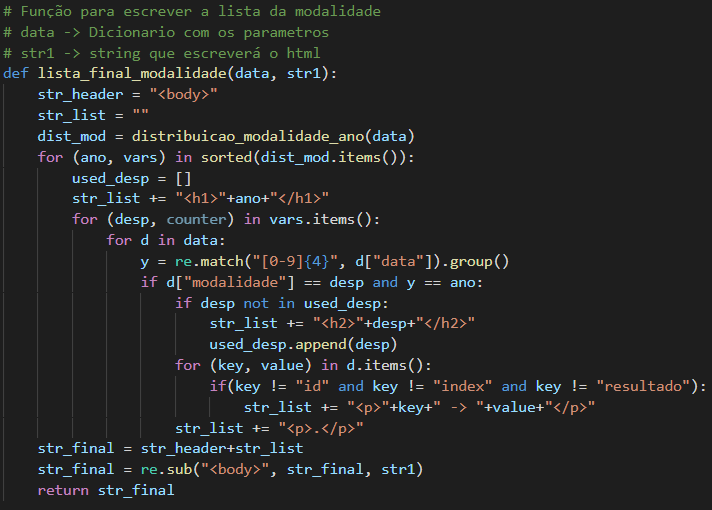
\includegraphics{lista_final_modalidade.png}}
\caption{Função lista\textunderscore final \textunderscore modalidade(data, str1)}
\label{fig}
\end{figure}  
As outras função são exatamente iguais a esta, só com o diferencial da ordenação dos dados.


\newpage
\subsection{Gerar HTMLs/Main} \label{subsec:htmlGenerator}
Numa primeira parte da main, criamos o "file descriptor" dos ficheiro csv.
Numa segunda parte, abrimos um ficheiro "index.html" onde será executado praticamente todo o código e criada a string para escrever o ficheiro html principal.
Após isto tudo, é criado todos as listas em html e em ficheiro separados seguindo a mesma lógica da string única para escrever tudo.


\begin{figure}[htbp]
\centerline{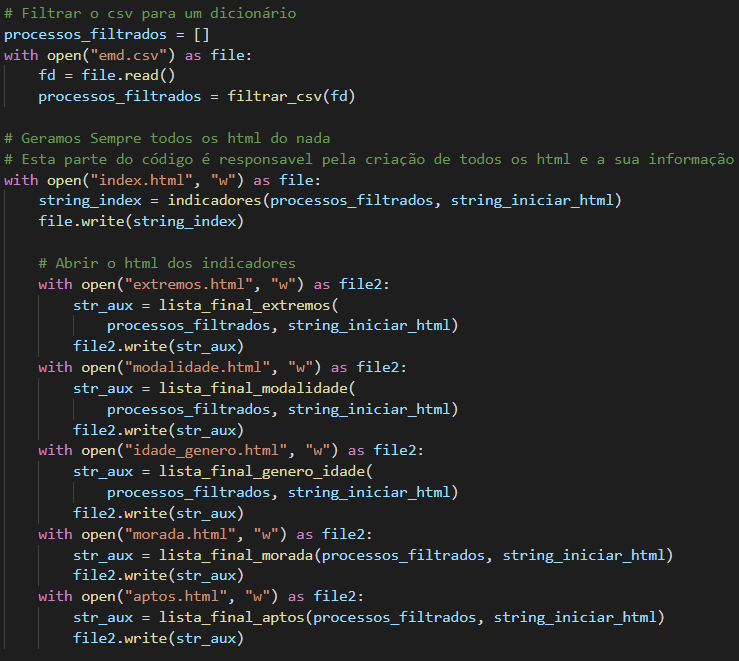
\includegraphics{gerar_html.png}}
\caption{Função gerar\textunderscore html (Main)}
\label{fig}
\end{figure}


\newpage
\section{Resultados do Problema 2} \label{sec:resProb2} %seccao e referencia cruzada
\subsection{Indicadores} \label{subsec:indc}
Aqui temos o ficheiro "index.html".

\begin{figure}[htbp]
\centerline{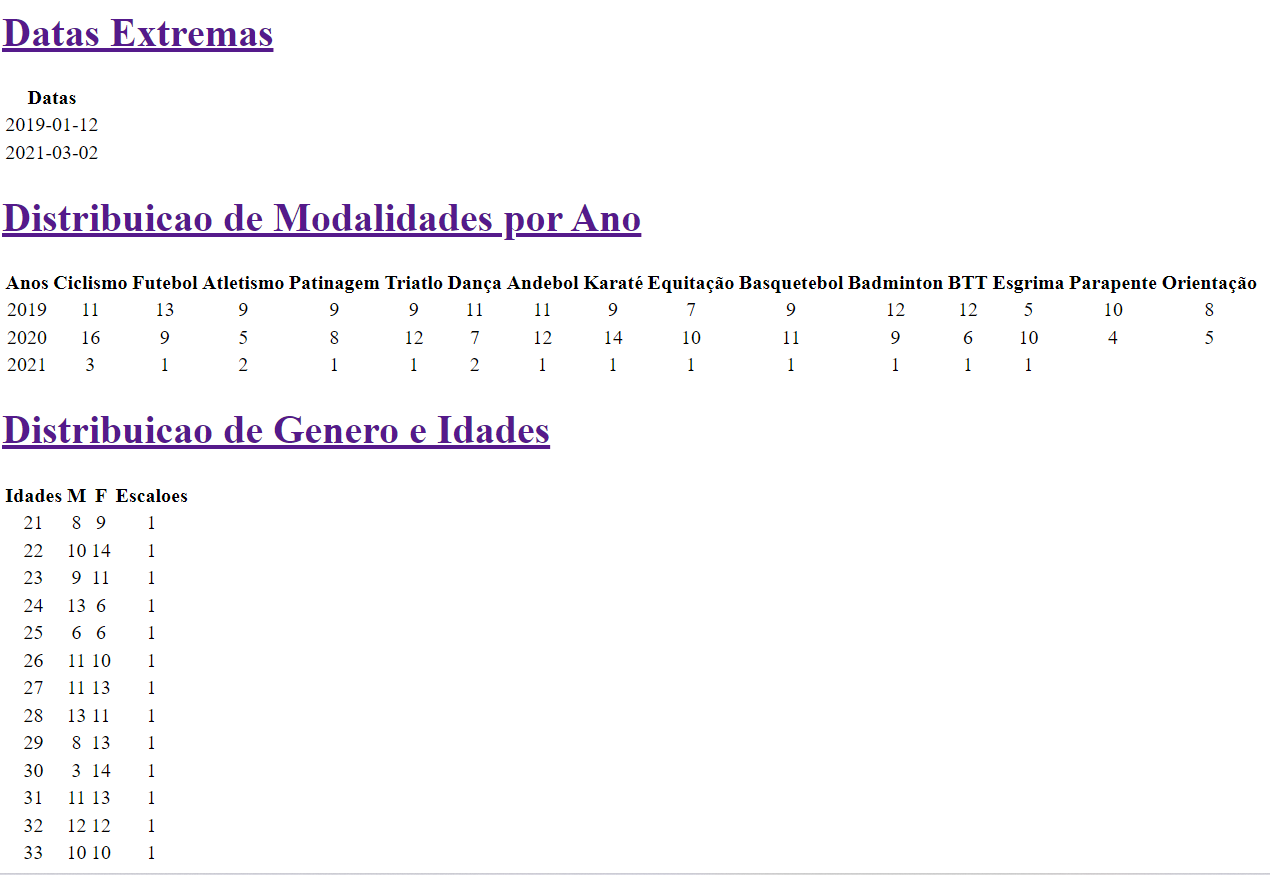
\includegraphics[scale=0.7]{index_html.png}}
\caption{Função index.html}
\label{fig}
\end{figure}
\newpage
\subsection{Exemplo de Listas} \label{subsec:exLista}
Aqui temos um exemplo de uma lista ao clicarmos no título do indicador em questão.
\begin{figure}[htbp]
\centerline{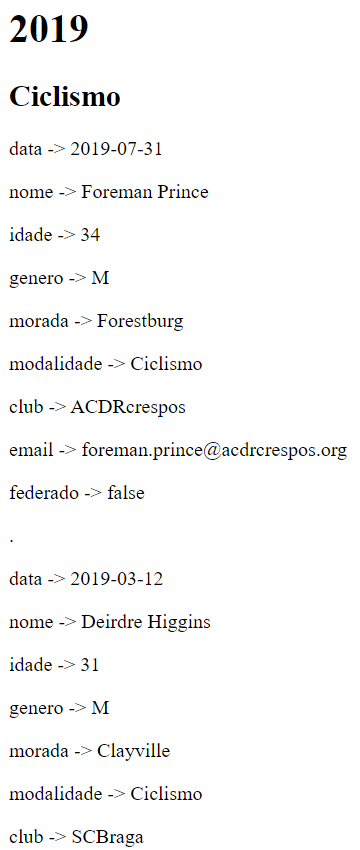
\includegraphics[scale=0.8]{modalidade_html.png}}
\caption{Função modalidade.html}
\label{fig}
\end{figure}

\chapter{Conclusão} \label{concl}
A realização deste trabalho prático possibilitou a consolidação da matéria lecionada sobre Expressões Regulares e processamento de texto, e também desenvolver mais conhecimentos sobre Python.\\
Em especifico este projeto permitiu-nos aprimorar a escrita de ER para resolução de problemas e filtragem de texto, bem como a a utilização do módulo 're' e as suas funções.\\
\appendix % apendice
\chapter{Código do Programa}
\subsection{Código do Exercício 1} \label{subsec:pyEx1}
\begin{verbatim}
import re

#Função para Filtrar Toda a informação e colocar-la num dicionário
def filtrar_info(fd):
    data_processos = []

    # Seperar por Linhas
    lista_newlines = fd.split("\n")

    # Seperar cada Linha em uma array com as informações
    for line in lista_newlines:
        if len(line):
            processos = line.split("::")

        # Dicionario default para colocar as informações
            dict_processo = {
                "Pasta": "",
                "Data": "",
                "Nome": "????",
                "Pai": "????",
                "Mae": "????",
                "Observacao": ""
            }


            # Filtrar o Processo:
            for parametro in processos:
                # Recolher a data
                if (re.match("[0-9]{4}-[0-9]{1,2}-[0-9]{1,2}", parametro)):
                    dict_processo["Data"] = parametro
                    continue
                # Recolher nr da Pasta
                if (re.match("[0-9]{1,4}", parametro)):
                    dict_processo["Pasta"] = parametro
                    continue
                # Recolher Informações que possuem Nomes Proprios (Começam por Letra maiscula)
                if (re.match("([A-Z]{1}[a-z]* ?)", parametro)):

                    if (re.search("[^A-Z]{1}\.", parametro)):
                        dict_processo["Observacao"] = parametro
                        continue
                    # Alocção ordenada de parametros ordenados:
                    if (dict_processo["Nome"] == "????"):
                        dict_processo["Nome"] = parametro
                        continue
                    if (dict_processo["Pai"] == "????"):
                        dict_processo["Pai"] = parametro
                        continue
                    if (dict_processo["Mae"] == "????"):
                        dict_processo["Mae"] = parametro
                        continue
                # Informação Inexistente
                if (re.match("", parametro)):
                    for (p1, p2) in dict_processo.items():
                        if dict_processo[p1] == "" or dict_processo[p1] == "????":
                            dict_processo[p1] = "!!NO INFO!!"
                            break

            data_processos.append(dict_processo)
    return data_processos


def calcular_freq_processos(data):
    dict_anos = {}
    total=0
    #Obter todos os processos por ano
    for processo in data:
        year = re.match("[0-9]{4}", processo["Data"]).group()
        if year not in dict_anos:
            dict_anos[year]=0
        total+=1
        dict_anos[year]+=1
    
    #Tabelar
    for (nome,counter) in sorted(dict_anos.items()):
        n = counter / total
        print("O ano tem "+str(nome) + " tem freq. de processos de:" + str(n))
    
    pass


# Falta descobrir o que está no "obs"
def calcular_freq_nomes_sec(data):
    #Variaveis Iniciais
    seculos = {}
    lista = ["Nome", "Pai", "Mae"]
    total_nomes_sec = {}
    total_apelidos_sec = {}

    #Ciclar toda a data e recolher toda a informação necessário para o exercício
    for processo in data:
        # Recolher o Ano e Fazer o Dicionario com o Seculo
        year = re.match("[0-9]{4}", processo["Data"]).group()
        year = int((int(year)-1) / 100)+1
        if (year not in seculos):
            seculos[year] = {"Primeiro_Nome": {}, "Apelido_Nome": {}}
            total_apelidos_sec[year] = 0
            total_nomes_sec[year] = 0

        # Recolher o Primeiro e o Ultimo Nome
        primeiro_nomes_lista = []
        apelidos_lista = []

        # Recolher Primerio e Ultimo Nome de Pai........
        for l in lista:
            if (processo[l] != "!!NO INFO!!"):
                primeiro_nome = re.search("^[A-Za-z]+", processo[l]).group()
                primeiro_nomes_lista.append(primeiro_nome)
                # Este if serve para os casos por exemplo "Ana Lopes Coelho (ou Ana Fernandes Lopes)"
                if (re.search("\)", processo[l])):
                    # Voltar a mandar o primeiro nome pra lista porque o Apelido é a unica coisa que difere
                    primeiro_nomes_lista.append(primeiro_nome)

                    # O apelido que está dentro de parentises
                    apelido_nome = re.search(
                        "[A-Za-z]*\)", processo[l]).group()[:-1]
                    apelidos_lista.append(apelido_nome)
                    # O apelido que está fora de parentises
                    apelido_nome = re.search(
                        "[A-Za-z]* \(", processo[l]).group()[:-2]
                    apelidos_lista.append(apelido_nome)
                else:
                    aux=processo[l]
                    #Em casos como: Maria Vale, Solteira
                    if (re.search(",", processo[l])):
                        aux=processo[l].split(",")[0]
                    apelido_nome = re.search("[A-Za-z]+$", aux).group()
                    apelidos_lista.append(apelido_nome)

        # Recolher Primerio e Ultimo Nome das observaçoes.
        if (processo["Observacao"] != "!!NO INFO!!"):
            obs_lista = re.findall(
                "(([A-Z]{1}[a-z]{1,} ?)+\,)", processo["Observacao"])
            #(nome,junk) pois a função findall está a criar um tuplo e nós queremos o primeiro membro
            for (nome, junk) in obs_lista:
                primeiro_nome = re.search("^[A-Za-z]+", nome[:-1]).group()
                primeiro_nomes_lista.append(primeiro_nome)
                apelido_nome = re.search("[A-Za-z]+$", nome[:-1]).group()
                apelidos_lista.append(apelido_nome)

        # Somar os Apelidos e Nomes de cada Seculo
        for n in primeiro_nomes_lista:
            if n not in seculos[year]["Primeiro_Nome"]:
                seculos[year]["Primeiro_Nome"][n] = 0
            total_nomes_sec[year] += 1
            seculos[year]["Primeiro_Nome"][n] += 1
        for n in apelidos_lista:
            if n not in seculos[year]["Apelido_Nome"]:
                seculos[year]["Apelido_Nome"][n] = 0
            total_apelidos_sec[year] += 1
            seculos[year]["Apelido_Nome"][n] += 1

    # Tabelar a Resposta:
    for (sec, data) in sorted(seculos.items()):
        print("Seculo: "+str(sec))
        print("\tNomes:")
        for (nome, counter) in data["Primeiro_Nome"].items():
            final = counter / total_nomes_sec[sec]
            print("\t\t"+str(nome)+" tem uma freq: "+str(final))
        print("\tApelidos:")
        for (nome, counter) in data["Apelido_Nome"].items():
            final = counter / total_nomes_sec[sec]
            print("\t\t"+str(nome)+" tem uma freq: "+str(final))
    return 0


def calcular_freq_relacao(data):
    #Criação de Variaveis
    total_relacoes =0
    dict_relacoes = {
        "Pai": 0,
        "Mae": 0
    }

    #Procurar as relações e somar las
    for processo in data:
        # Ver se o Pai ou Mae existe (podem ser desconhecido)
        if (processo["Pai"] != "!!NO INFO!!"):
            dict_relacoes["Pai"]+=1
            total_relacoes+=1

        if (processo["Mae"] != "!!NO INFO!!"):
            total_relacoes+=1
            dict_relacoes["Mae"]+=1

        #Relações que estão na observação
        relacoes = re.findall("[^A-Z]\,(([A-Z]{1}[a-z ]+)+)\.",processo["Observacao"])
        if(relacoes):
            relacoes = relacoes[0][0]

            #Tivemos de Adicionar estas 2 Excluisoes, pois eles sairam fora do nosso ER, Somente estes 2 casos!
            if not(re.match("Jeronimo Silva Coelho", relacoes) or re.match("Frei", relacoes)):
                if (relacoes not in dict_relacoes):
                    dict_relacoes[relacoes] =0 
                dict_relacoes[relacoes]+=1
                total_relacoes+=1

    #Criar a Tabela:
    print("Frequencias de Relacoes: ")
    for (rel,counter) in dict_relacoes.items():
        freq = counter/total_relacoes
        print("\tA relação "+str(rel)+" tem de freq: " +str(freq))


    return 0


#Criar o JSON
def criar_json(data,n):
    lista=[]
    counter=0
    for d in data:
        lista.append(d)
        if(counter > n-2):
            break
        counter+=1
    return lista

#Função para abrir o processos
with open('processos.txt') as file:
    #Abrir o file descriptor
    fd = file.read()
    #Colocar os processos na estrutura de dados
    processos_filtrados = filtrar_info(fd)

    #Criar um Menu e escolher a opção
    x = int(input("Digite qual exercicio:\n1-> Frequencia de Processos por Ano\n2-> Frequencia de Nomes Proprios e Apelidos por Seculo\n3-> Frequencia dos Tipos de Relação\nOpcao: "))
    if (x == 1):
        calcular_freq_processos(processos_filtrados)
    elif(x == 2):
        calcular_freq_nomes_sec(processos_filtrados)
    elif(x == 3):
        calcular_freq_relacao(processos_filtrados)

    #Criar o ficheiro JSON
    with open('processos.json', 'w') as file_output:
        dados_json= criar_json(processos_filtrados,20)
        file_output.write(str(dados_json))
\end{verbatim}

\subsection{Código do Exercício 2} \label{subsec:pyEx2}
\begin{verbatim}
import re

string_iniciar_html = '<!DOCTYPE html><html lang="en"><head><meta charset="UTF-8"><meta http-equiv="X-UA-Compatible" content="IE=edge"><meta name="viewport" content="width=device-width, initial-scale=1.0"><title>Document</title></head><body></body></html>'


# Função Inicial para filtrar toda a informação para um dicionário
def filtrar_csv(fd):
    lista_newlines = fd.split("\n")
    data = []
    counter = 0
    # Seperar cada Linha em uma array com as informações
    for line in lista_newlines:
        # Dicionario para colocar a info do CSV
        dict_processo = {
            "id": "",
            "index": "",
            "data": "",
            "nome": "",
            "idade": "",
            "genero": "",
            "morada": "",
            "modalidade": "",
            "club": "",
            "email": "",
            "federado": "",
            "resultado": ""
        }
        if(line and counter > 0):
            # Colocar a Informação do dicionario apos uma pequena verificação
            row = line.split(",")
            if (re.match("[0-9a-z]{24}", row[0])):
                dict_processo["id"] = row[0]
            if (re.match("[0-9]{1,2}", row[1])):
                dict_processo["index"] = row[1]
            if (re.match("[0-9]{4}-[0-9]{1,2}-[0-9]{1,2}", row[2])):
                dict_processo["data"] = row[2]
            if (re.match("[A-Za-z]+", row[3])):
                dict_processo["nome"] = row[3]
            if (re.match("[A-Za-z]+", row[4])):
                dict_processo["nome"] += " "+row[4]
            if (re.match("[0-9]{2}", row[5])):
                dict_processo["idade"] = row[5]
            if (re.match("[MF]{1}", row[6])):
                dict_processo["genero"] = row[6]
            if (re.match("[A-Za-z]+", row[7])):
                dict_processo["morada"] = row[7]
            if (re.match("[A-Za-z]+", row[8])):
                dict_processo["modalidade"] = row[8]
            if (re.match("[A-Za-z]+", row[9])):
                dict_processo["club"] = row[9]
            if (re.match("[a-zA-Z.]+@[a-zA-Z.]+", row[10])):
                dict_processo["email"] = row[10]
            if (re.match("true|false", row[11])):
                dict_processo["federado"] = row[11]
            if (re.match("true|false", row[12])):
                dict_processo["resultado"] = row[12]
        if (dict_processo["id"] != ""):
            data.append(dict_processo)
        counter += 1
    return data


# Função que devolve as datas mais extremas do nosso CSV
def datas_extremas(data):
    # Obter todas as datas numa lista e ordenar por ano -> mes -> dia
    aux_list = []
    for d in data:
        n = d["data"].split("-")
        aux_list.append(n)
        aux_list = sorted(aux_list, key=lambda i: (i[0], i[1], i[2]))

    # Passar os extremos para strings
    menor_data = aux_list.pop(0)
    menor_data_str = ""
    for i in menor_data:
        menor_data_str += i+"-"

    maior_data = aux_list.pop(-1)
    maior_data_str = ""
    for i in maior_data:
        maior_data_str += i+"-"

    return (menor_data_str[:-1], maior_data_str[:-1])


# Função que devolve um dicionário com cada modalidade por ano
def distribuicao_modalidade_ano(data):
    dict_distribuicao = {}
    for d in data:
        #obter o ano da data
        year = re.match("[0-9]{4}", d["data"]).group()
        #Obter a distribuição por modalidade
        if year not in dict_distribuicao:
            dict_distribuicao[year] = {}
        if d["modalidade"] not in dict_distribuicao[year]:
            dict_distribuicao[year][d["modalidade"]] = 0
        dict_distribuicao[year][d["modalidade"]] += 1

    return dict_distribuicao


# Função que devolve um dicionário com idades, generos e os escalões
def distribuicao_genero_idade(data):
    dict_distribuicao = {}
    for d in data:
        #obter a distribuição por genero e idade
        if d["idade"] not in dict_distribuicao:
            dict_distribuicao[d["idade"]] = {}
            dict_distribuicao[d["idade"]]["M"] = 0
            dict_distribuicao[d["idade"]]["F"] = 0
        dict_distribuicao[d["idade"]][d["genero"]] += 1
        # Obter os escaloes
        if (int(d["idade"]) < 35):
            dict_distribuicao[d["idade"]]["Escaloes"] = 1
        else:
            dict_distribuicao[d["idade"]]["Escaloes"] = 2
    return dict_distribuicao


# Função que devolve um dicionário com as moradas
def distribuicao_morada(data):
    dict_distribuicao = {}
    for d in data:
        #Obter a distribuição por modalidade
        if d["morada"] not in dict_distribuicao:
            dict_distribuicao[d["morada"]] = 0
        dict_distribuicao[d["morada"]] += 1
    return dict_distribuicao


# Função para calcular os atletas que estão aptos ou não
def aptos(data):
    dict_distribuicao = {}
    for d in data:
        #Obter o ano da Data
        year = re.match("[0-9]{4}", d["data"]).group()
        #Obter a distribuição por modalidade
        if year not in dict_distribuicao:
            dict_distribuicao[year] = {}
        if d["resultado"] not in dict_distribuicao[year]:
            dict_distribuicao[year][d["resultado"]] = 0
        dict_distribuicao[year][d["resultado"]] += 1

    # Calcular o Total para a percentagem:
    for year in dict_distribuicao:
        counter = 0
        for (key, value) in dict_distribuicao[year].items():
            counter += value
        if("true" in dict_distribuicao[year] and "false" in dict_distribuicao[year]):
            dict_distribuicao[year]["true"] = str(
                dict_distribuicao[year]["true"]/counter)+"  %"
            dict_distribuicao[year]["false"] = str(
                dict_distribuicao[year]["false"]/counter)+" %"
    return dict_distribuicao


# Função para escrever tabelas recebendo:
# data -> Dicionario com os parametros
# str1 -> string que escreverá o html
# nome_tabela -> String que dá o nome ao "h1" do html
# p_header -> String que dá o titulo à primeira coluna das tabelas
# anchor -> String com o path para o html
def draw_table_html(data, str1, nome_tabela, p_header, anchor):
    used_key = []
    str_header = '<body><h1><a href='+anchor+">"+nome_tabela + \
        '</a></h1><table><tr><th style="text-align: center">'+p_header+'</th>'
    str_table = ""
    for (year, var) in sorted(data.items()):
        str_table += '<tr><td style="text-align: center">'+str(year)+"</td>"
        for (key, value) in var.items():
            if key not in used_key:
                used_key.append(key)
                str_header += '<th style="text-align: center">' + \
                    str(key)+"</th>"
            str_table += '<td style="text-align: center">'+str(value)+"</td>"
        str_table += "</tr>"
    str_header += "</tr>"
    str_table += "</table>"
    str_final = re.sub("<body>", str_header+str_table, str1)

    return str_final

# Função "igual" à draw_table_html
# Esta teve de ser diferente pois é um dicionario bem mais simples
def draw_table_html_morada(data, str1, nome_tabela):
    str_header = '<body><h1><a href="morada.html">'+nome_tabela + \
        '</a></h1><table><tr><th style="text-align: center">Moradas</th><th style="text-align: center">Numero de Habitantes</th>'
    str_table = ''
    for (morada, value) in sorted(data.items()):
        str_table += '<tr><td style="text-align: center">'+str(morada)+'</td>'
        str_table += '<td style="text-align: center">'+str(value)+"</td></tr>"
    str_header += "</tr>"
    str_table += "</table>"
    str_final = re.sub("<body>", str_header+str_table, str1)
    return str_final


# Função para escrever os extremos no html
def data_extremas_html(datas, str1):
    str_header = '<body><h1><a href="extremos.html">Datas Extremas</a></h1><table><tr><th style="text-align: center">Datas</th>'
    str_table = '<tr><td style="text-align: center">'+str(datas[0])+'</td>'
    str_table += '<tr><td style="text-align: center">'+str(datas[1])+'</td>'
    str_header += "</tr>"
    str_table += "</table>"
    str_final = re.sub("<body>", str_header+str_table, str1)
    return str_final


# Função com os indicadores estatisticos
def indicadores(data, str1):
    datas_extremas_result = datas_extremas(data)
    distribuicao_modalidade_ano_result = distribuicao_modalidade_ano(data)
    distribuicao_genero_idade_result = distribuicao_genero_idade(data)
    distribuicao_morada_result = distribuicao_morada(data)
    aptos_result = aptos(data)

    # Desenhar as Tabelas no index.html
    str1 = draw_table_html_morada(
        distribuicao_morada_result, str1, "Distribuicao de Moradas")
    str1 = draw_table_html(
        aptos_result, str1, "Percentagem de Aptos", "Anos", "aptos.html")
    str1 = draw_table_html(distribuicao_genero_idade_result,
                           str1, "Distribuicao de Genero e Idades", "Idades", "idade_genero.html")
    str1 = draw_table_html(distribuicao_modalidade_ano_result,
                           str1, "Distribuicao de Modalidades por Ano", "Anos", "modalidade.html")
    str1 = data_extremas_html(datas_extremas_result, str1)
    return str1


# Função para escrever a lista da modalidade
# data -> Dicionario com os parametros
# str1 -> string que escreverá o html
def lista_final_modalidade(data, str1):
    str_header = "<body>"
    str_list = ""
    dist_mod = distribuicao_modalidade_ano(data)
    for (ano, vars) in sorted(dist_mod.items()):
        used_desp = []
        str_list += "<h1>"+ano+"</h1>"
        for (desp, counter) in vars.items():
            for d in data:
                y = re.match("[0-9]{4}", d["data"]).group()
                if d["modalidade"] == desp and y == ano:
                    if desp not in used_desp:
                        str_list += "<h2>"+desp+"</h2>"
                        used_desp.append(desp)
                    for (key, value) in d.items():
                        if(key != "id" and key != "index" and key != "resultado"):
                            str_list += "<p>"+key+" -> "+value+"</p>"
                    str_list += "<p>.</p>"
    str_final = str_header+str_list
    str_final = re.sub("<body>", str_final, str1)
    return str_final

# Função para escrever a lista do genero/idade
def lista_final_genero_idade(data, str1):
    used_idade = []
    str_header = "<body>"
    str_list = ""
    dist_genero = distribuicao_genero_idade(data)
    for (idade, vars) in sorted(dist_genero.items()):
        for d in data:
            if d["idade"] == idade:
                if idade not in used_idade:
                    str_list += "<h2>"+idade+" Anos </h2>"
                    used_idade.append(idade)
                for (key, value) in d.items():
                    if(key != "id" and key != "index" and key != "resultado"):
                        str_list += "<p>"+key+" -> "+value+"</p>"
                str_list += "<p>.</p>"
    str_final = str_header+str_list
    str_final = re.sub("<body>", str_final, str1)
    return str_final

# Função para escrever a lista das datas extremas
def lista_final_extremos(data, str1):
    str_header = "<body>"
    str_list = ""
    extremos = datas_extremas(data)
    for d in data:
        if (d["data"] == extremos[0] or d["data"] == extremos[1]):
            str_list += "<h1>"+ d["data"] + "</h1>"
            for (key, value) in d.items():
                if(key != "id" and key != "index" and key != "resultado"):
                    str_list += "<p>"+key+" -> "+value+"</p>"
            str_list += "<p>.</p>"
    str_final = str_header+str_list
    str_final = re.sub("<body>", str_final, str1)
    return str_final 

# Função para escrever a lista dos aptos
def lista_final_aptos(data, str1):
    str_header = "<body>"
    str_list = ""
    for d in data:
        for (key, value) in d.items():
            if(key != "id" and key != "index" and key != "resultado"):
                str_list += "<p>"+key+" -> "+value+"</p>"
        str_list += "<p>.</p>"
    str_final = str_header+str_list
    str_final = re.sub("<body>", str_final, str1)
    return str_final

# Função para escrever a lista das moradas
def lista_final_morada(data, str1):
    used_name = []
    str_header = "<body>"
    str_list = ""
    dist_moradas = distribuicao_morada(data)
    for (morada, counter) in sorted(dist_moradas.items()):
        for d in data:
            if d["morada"] == morada:
                if morada not in used_name:
                    str_list += "<h2>"+morada+"</h2>"
                    used_name.append(morada)
                for (key, value) in d.items():
                    if(key != "id" and key != "index" and key != "resultado"):
                        str_list += "<p>"+key+" -> "+value+"</p>"
                str_list += "<p>.</p>"
    str_final = str_header+str_list
    str_final = re.sub("<body>", str_final, str1)
    return str_final


# Filtrar o csv para um dicionário
processos_filtrados = []
with open("emd.csv") as file:
    fd = file.read()
    processos_filtrados = filtrar_csv(fd)

# Geramos Sempre todos os html do nada
# Esta parte do código é responsavel pela criação de todos os html e a sua informação
with open("index.html", "w") as file:
    string_index = indicadores(processos_filtrados, string_iniciar_html)
    file.write(string_index)

    # Abrir o html dos indicadores
    with open("extremos.html", "w") as file2:
        str_aux = lista_final_extremos(
            processos_filtrados, string_iniciar_html)
        file2.write(str_aux)
    with open("modalidade.html", "w") as file2:
        str_aux = lista_final_modalidade(
            processos_filtrados, string_iniciar_html)
        file2.write(str_aux)
    with open("idade_genero.html", "w") as file2:
        str_aux = lista_final_genero_idade(
            processos_filtrados, string_iniciar_html)
        file2.write(str_aux)
    with open("morada.html", "w") as file2:
        str_aux = lista_final_morada(processos_filtrados, string_iniciar_html)
        file2.write(str_aux)
    with open("aptos.html", "w") as file2:
        str_aux = lista_final_aptos(processos_filtrados, string_iniciar_html)
        file2.write(str_aux)

\end{verbatim}

\end{document} 
